% Dokumentum konfiguráció
\documentclass[fleqn,12pt]{article}
% --------------------------------------------------
% Dokumentum adatok
% --------------------------------------------------

% Intézmény és kar
\newcommand\INTEZMENY{Budapesti Műszaki és Gazdaságtudományi Egyetem}
\newcommand\KAR{Gépészmérnöki Kar}
\newcommand\LOGO{bme-logo.jpg} % logo fájl neve a figures mappában

% Dokumentum adatok
\newcommand\CIM{Dinamika 1. házi feladat}
\newcommand\DATUM{2026/27 I.}
\newcommand\NEV{Abos Gergő}
\newcommand\NEPTUN{C46M9M}
\newcommand\EMAIL{gergo.abos@gmail.com}
\newcommand\TANTARGY{Dinamika}
\newcommand\TANTARGYKOD{BMEGEMMBXM3}

% --------------------------------------------------
% Preambulum és egyéni parancsok betöltése
% --------------------------------------------------

% --------------------------------------------------
% Fájl: 00_preambulum.tex
% --------------------------------------------------

% --------------------------------------------------
% Packagek
% --------------------------------------------------

% Dokumentum konfiguráció
\usepackage[hungarian]{babel} % dokumentum nyelvi beállítása
\usepackage[utf8]{inputenc} % bemeneti betűkódolás (ékezetes karakterek)
\usepackage[T1]{fontenc} % kimeneti betűkódolás (ékezetes karakterek)
\usepackage{lmodern} % bővített karakterkészlet az ékezetekhez
\usepackage{geometry} % dokumentum margók és oldalbeállítások
\usepackage{hyperref} % hivatkozások és linkek
\usepackage[backend=biber,style=numeric,sorting=none]{biblatex} % irodalomjegyzék

% Ábrák, grafikák
\usepackage{graphicx} % klépek beillesztése és méretezése
\usepackage{float} % ábrák és táblázatok elhelyezésének pontos szabályozása
\usepackage{caption} % képaláírások formázása
\usepackage{tikz} % vektorgrafikák, ábrák rajzolása LaTeX-ben
\usepackage{xcolor} % színek kezelése

\usepackage{pdfpages} % teljes PDF-oldalak beillesztése a dokumentumba

% Matematikai és fizikai írásmód
\usepackage{amsmath,amsthm,amsfonts,amssymb,amscd} % matematikai környezetek és szimbólumok
\usepackage{mathtools} % kiegészítő matematikai eszközök az amsmath-hoz
\usepackage{siunitx} % SI mértékegységek helyes jelölése

% Fejléc, lábléc
\usepackage{fancyhdr} % egyedi fejléc és lábléc készítése
\usepackage{lastpage} % az utolsó oldal sorszámának hivatkozása

% Dokumentumtagolás
\usepackage{titlesec} % címsorok formázásának testreszabása
\usepackage{csquotes} % idézetek helyes formázása (nyelvspecifikus)
\usepackage{booktabs} % szép, tipográfiailag helyes táblázatok készítése
\usepackage{float}

% --------------------------------------------------
% Dokumentum beállítások
% --------------------------------------------------

% Dokumentum formátum
\geometry{a4paper,total={170mm,240mm},left=20mm,top=30mm} % oldalbeállítások: A4, margók méretezése
\setlength\parindent{0pt} % bekezdések behúzásának kikapcsolása

% Fejléc, lábléc beállítása
\pagestyle{fancy} % fancyhdr csomag stílus használata
\renewcommand{\headrulewidth}{0.4pt} % fejléc vonalvastagsága
\renewcommand{\footrulewidth}{0.4pt} % lábléc vonalvastagsága
\headheight 1.5em % fejléc magasságának beállítása
\rhead{\NEV{}, \NEPTUN{}} % job\mathbf{B}felső sarok
\chead{} % középső fejléc
\lhead{\TANTARGYKOD{}, \TANTARGY{}} % bal felső sarok
\lfoot{} % bal alsó sarok
\cfoot{\small\thepage} % középső lábléc
\rfoot{} % jobb alsó sarok
\headsep 1.5em % fejléc és szöveg közötti távolság

% Hyperref beállítások - PDF megjelenítés
\hypersetup{
  colorlinks=true, % színes linkek
  linkcolor=blue, % belső hivatkozások színe
  urlcolor=cyan, % URL hivatkozások színe
  pdftitle={\CIM{}}, % PDF cím
  pdfauthor={\NEV{}}, % PDF szerző
  pdfsubject={\TANTARGY{} (\TANTARGYKOD{})}, % PDF tárgy
  bookmarksopen=true, % könyvjelzők alapból nyitva
  bookmarksnumbered=true, % könyvjelzők számozása
  pdfpagemode=UseOutlines % könyvjelzők megjelenítése PDF olvasóban
}

% Irodalomjegyék beállítása
% \addbibresource{contents/literature.bib} % irodalomjegyzék forrásfájl

% Számozások beállítása fejezetenként
% \numberwithin{equation}{section} % egyenletek számozása fejezetenként
% \numberwithin{figure}{section} % ábrák számozása fejezetenként
% \numberwithin{table}{section} % táblázatok számozása fejezetenként

% Táblázat formátum beállítása - Függőlegesen középre igazított szöveg
\newcolumntype{L}[1]{>{\raggedright\let\newline\\\arraybackslash\hspace{0pt}}m{#1}} % balra zárt
\newcolumntype{C}[1]{>{\centering\let\newline\\\arraybackslash\hspace{0pt}}m{#1}} % középre zárt
\newcolumntype{R}[1]{>{\raggedleft\let\newline\\\arraybackslash\hspace{0pt}}m{#1}} % jobbra zárt
\renewcommand{\arraystretch}{1.25} % táblázatok sormagassága

% Mértékegységek formátuma
\sisetup{exponent-product = \cdot, per-mode=fraction} % SI jelölések

% Tikz
\usetikzlibrary{math} % matematikai számítások Tikz-ben
\usetikzlibrary{calc} % geometriai számítások (pl. koordináták)
\usetikzlibrary{angles} % szögjelölések rajzolása
\usetikzlibrary{quotes} % címkék és feliratok egyszerű kezelése
\usetikzlibrary{arrows.meta} % nyílstílusok
\usetikzlibrary{patterns}
\usetikzlibrary{decorations, decorations.markings}  

% --------------------------------------------------
% Fájl: 01_commands.tex
% --------------------------------------------------

% --------------------------------------------------
% Matematikai parancsok
% --------------------------------------------------

% Általános matematikai parancsok
\renewcommand{\d}[1]{\mathrm{d}#1} % differenciál jel
\renewcommand{\vec}[1]{\mathbf{#1}} % vektor jelölés
\newcommand{\norm}[1]{\left\lVert #1 \right\rVert} % norma
\newcommand{\abs}[1]{\left\lvert #1 \right\rvert} % abszolút érték

% Lineár algebrai műveletek
\DeclareMathOperator{\rank}{rank} % rang
\DeclareMathOperator{\tr}{tr} % nyom (trace)
\DeclareMathOperator{\diag}{diag} % diagonális mátrix

% Vektoranalízis műveletek
\DeclareMathOperator{\grad}{\mathbf{grad}} % grad
\DeclareMathOperator{\rot}{\mathbf{rot}} % rot
\DeclareMathOperator{\diverg}{\mathbf{div}} % div
\DeclareMathOperator{\laplace}{\Delta} % Laplace-operátor

% Egyé\mathbf{B}műveletek
\newcommand{\eval}[2]{\left. #1 \right|_{#2}} % kifejezés kiértékelése

% --------------------------------------------------
% Egyé\mathbf{B}parancsok
% --------------------------------------------------

\newcommand*\circled[1]{
  \begin{tikzpicture}[baseline=(C.base)] \node[draw,circle,inner sep=2pt](C) {#1};
\end{tikzpicture}} % karikázás

% Abos Gergő parancsai:
\newcommand{\figref}[1]{\hyperref[#1]{Abb.~\ref*{#1}}}

%%%%%%%%%%%%%%%%%%%%%%%%%%%%%%%%%%%%%%%%%%%%%%%%%%%%
% mechTikz - Rúd szerkezetek rajzolása TikZ segítségével
%%%%%%%%%%%%%%%%%%%%%%%%%%%%%%%%%%%%%%%%%%%%%%%%%%%%

% --------------------------------------------------
% Alapstílusok
% --------------------------------------------------
% Definiáljuk a gyakran használt TikZ stílusokat
% (pl. pontok, rudak, erővektorok, stb.)

\tikzset{
  point/.style = {circle,fill=black,inner sep = 1.5pt},
  link/.style = {color=#1, very thick},
  angle/.style={color=#1,<->, >=latex},
  vec/.style = {color=#1,very thick,-latex},
  arc vec/.style={color=#1,very thick, postaction={decorate}, decoration={markings,mark=at position 1 with {\arrow{>}}}},
  arc vec2/.style={color=#1,very thick, postaction={decorate}, decoration={markings,mark=at position 1 with {\arrow{<}}}},
  force/.style = {color=red, very thick, ->},
  moment/.style = {color=#1,very thick,-Implies, double distance=1pt},
  coordSys/.style = {color=#1, thin,-latex},
  guide/.style = {color=#1,thin},
  guideVec/.style = {color=#1,latex-latex},
  construct/.style = {color=#1,thick,dashed},
  support/.style={link={black}, fill=white},
  > = Stealth
}

%%%%%%%%%%%%%%%%%%%%%%%%%%%%%%%%%%%%%%%%%%%%%%%%%%%%
% Saját TikZ parancsok definiálása
%%%%%%%%%%%%%%%%%%%%%%%%%%%%%%%%%%%%%%%%%%%%%%%%%%%%
% Ezek a parancsok új "rajzelemeket" hoznak létre,
% amiket később egyszerűen, rövid paranccsal hívhatunk
% meg rajzolás közben (pl. \supporthinge{A}{0}).

% --------------------------------------------------
% Általános elemek
% --------------------------------------------------

% Távolságjelölő makró
\newcommand{\dimarrow}[7][]{%
  % #1: opcionális TikZ stílus (pl. color=red, thick, stb.)
  % #2: első pont
  % #3: második pont
  % #4: eltolás vektor 1 (pl. (0,-1.25) vagy (1,0))
  % #5: eltolás vektor 2 (pl. (0,-1.25) vagy (1,0))
  % #6: felirat a nyíl közepén
  % #7: felirat pozíció (pl. below, above, left, right)
  \begin{scope}[#1]
    % vezető vonalak
    \draw[guide={gray}] ($(#2)+#4$) -- (#2);
    \draw[guide={gray}] ($(#3)+#5$) -- (#3);
    % távolság nyíl felirattal
    \draw[guideVec={gray}] ($(#2)+#4$) -- node[midway, #7] {#6} ($(#3)+#5$);
  \end{scope}
}

% Kis koordinátarendszer megrajzolása
\newcommand{\coordSys}[2][]{%
  % #1: opcionális paraméter (pl. scale=1.2, draw=blue, stb.)
  % #2: csomópont koordinátája (pl. (2,3))
  \begin{scope}[shift={(#2)}, #1]
    % x tengely
    \draw[coordSys={red}] (-0.5,0) -- (0.5,0) node[right] {$x$};
    % y tengely
    \draw[coordSys={red}] (0,-0.5) -- (0,0.5) node[above] {$y$};
  \end{scope}
}

% --------------------------------------------------
% Mechanikai elemek
% --------------------------------------------------

% Csuklós alátámasztás + ground
\newcommand{\supporthinge}[3][]{%
  % #1: opcionális paraméter (pl. scale=1.2, draw=blue, stb.)
  % #2: csomópont koordinátája
  % #3: forgatási szög fokban
  \begin{scope}[shift={(#2)}, rotate=#3, #1]
    % Talaj
    \fill[gray!20!white] (-0.5,-0.5) rectangle (0.5,-0.75);
    \draw[black, very thick] (-0.5,-0.5) -- (0.5,-0.5);
    % Háromszög
    \draw[support] (0,0) -- (-0.25,-0.5) -- (0.25,-0.5) -- cycle;
    \fill[white, draw={black}] (0,0) circle (0.1cm);
  \end{scope}
}

% Görgős alátámasztás + ground
\newcommand{\supportroller}[3][]{%
  % #1: opcionális paraméter
  % #2: csomópont koordinátája
  % #3: forgatási szög fokban
  \begin{scope}[shift={(#2)}, rotate=#3, #1]
    % Talaj
    \fill[gray!20!white] (-0.5,-0.5) rectangle (0.5,-0.75);
    \draw[black, very thick] (-0.5,-0.5) -- (0.5,-0.5);
    % Háromszög + görgők
    \draw[support] (0,0) -- (-0.25,-0.35) -- (0.25,-0.35) -- cycle;
    \foreach \i in {-0.15,0,0.15} {
      \draw[support] (\i,-0.425) circle (0.075);
    }
    \fill[white, draw={black}] (0,0) circle (0.1cm);
  \end{scope}
}

% Befogás
\newcommand{\supportfixed}[3][]{%
  % #1: opcionális paraméter (pl. line width, color, stb.)
  % #2: csomópont koordinátája
  % #3: forgatási szög fokban
  \begin{scope}[shift={(#2)}, rotate=#3, #1]
    % Talaj (befogás jelölés)
    \fill[gray!20!white] (-0.5,0) rectangle (0.5,-0.5);
    \draw[black, very thick] (-0.5,0) -- (0.5,0);
  \end{scope}
}

% Csúszka
\newcommand{\supportslider}[4][]{%
  % #1: opcionális paraméter (pl. line width, color, stb.)
  % #2: csomópont koordinátája
  % #3: forgatási szög fokban
  % #4: sín szélessége (alapértelmezett: 1)
  \begin{scope}[shift={(#2)}, rotate=#3, #1]
    % Felső sín
    \fill[gray!20!white] (-0.75,#4/2) rectangle (0.75,#4/2+0.25);
    \draw[black, very thick] (-0.75,#4/2) -- (0.75,#4/2);
    % Alsó sín
    \fill[gray!20!white] (-0.75,-#4/2) rectangle (0.75,-#4/2-0.25);
    \draw[black, very thick] (-0.75,-#4/2) -- (0.75,-#4/2);
  \end{scope}
}

% Kötél kényszer
\newcommand{\supportrope}[4][]{%
  % #1: opcionális paraméter (pl. scale, color, stb.)
  % #2: csomópont koordinátája
  % #3: forgatási szög fokban (pl. ha nem függőleges kábelt akarsz)
  \begin{scope}[shift={(#2)}, rotate=#3, #1]
    % Talaj (felfogatási pont)
    \fill[gray!20!white] (-0.5,-#4-0.25) rectangle (0.5,-#4-0.5);
    \draw[black, very thick] (-0.5,-#4-0.25) -- (0.5,-#4-0.25);
    % Kötél
    \draw[black, thick, densely dashed] (0,0) -- (0,-#4-0.25);
    % Pontok
    \fill[black] (0,-#4-0.25) circle (0.05); % alsó pont
    \fill[black] (0,0) circle (0.05);        % felső pont
  \end{scope}
}

% Sima támasz + ground
\newcommand{\supportsimple}[3][]{%
  % #1: opcionális paraméter (pl. scale=1.2, draw=blue, stb.)
  % #2: csomópont koordinátája
  % #3: forgatási szög fokban
  \begin{scope}[shift={(#2)}, rotate=#3, #1]
    % Talaj
    \fill[gray!20!white] (-0.5,-0.5) rectangle (0.5,-0.75);
    \draw[black, very thick] (-0.5,-0.5) -- (0.5,-0.5);
    % Félkör támasz
    \draw[support] (0.25,-0.25) arc[start angle=0, end angle=180, radius=0.25];
    % Oldalsó vonalak a félkörhöz
    \draw[support] (-0.25,-0.25) -- (-0.25,-0.5) (0.25,-0.5) -- (0.25,-0.25) -- cycle;
  \end{scope}
}

% Csukló
\newcommand{\hinge}[2][]{%
  % #1: opcionális paraméter (pl. scale=1.2, draw=blue, stb.)
  % #2: csomópont koordinátája
  \begin{scope}[shift={(#2)}, #1]
    \fill[white, draw={black}] (0,0) circle (0.1cm);
  \end{scope}
}


% ==================================================
% Dokumentum kezdete
% ==================================================
\begin{document}

% Címlap és tartalomjegyzék
% \input{contents/01_title.tex}
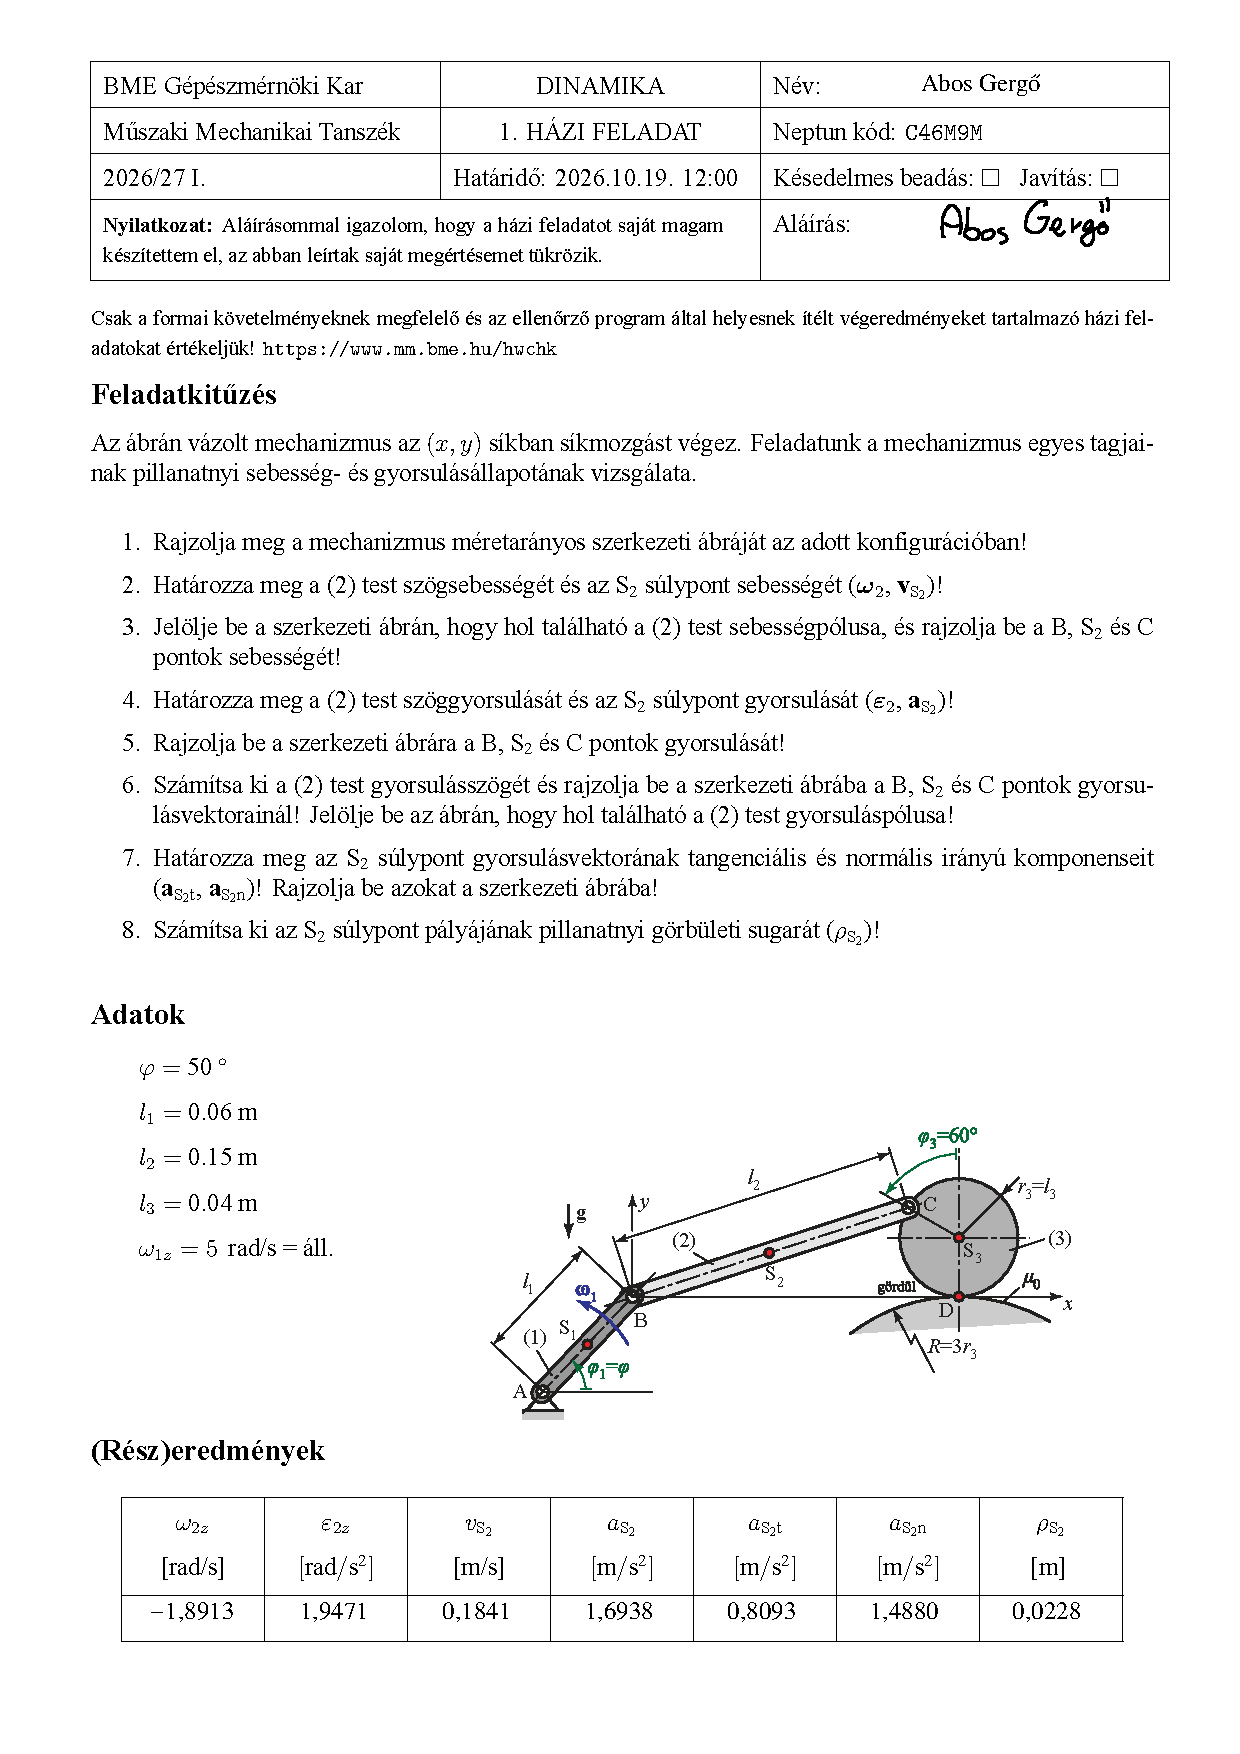
\includepdf[pages=1]{contents/Taskpage_filled.pdf}

\section{Méretarányos szerkezeti ábra}
\begin{figure}[H]
    \centering
    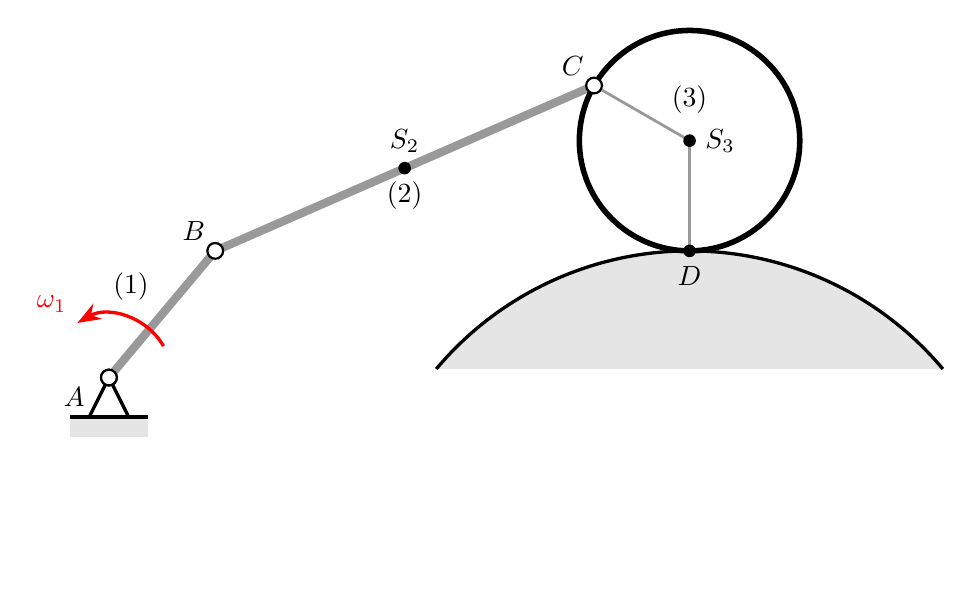
\begin{tikzpicture}[>=Stealth, thick]
    \def\sc{35} % Scale factor
    
    \coordinate (A) at (0*\sc, 0*\sc);
    \coordinate (B) at (0.03857*\sc, 0.04596*\sc);
    \coordinate (C) at (0.17604*\sc, 0.10596*\sc);
    \coordinate (S3) at (0.21069*\sc, 0.08596*\sc);
    \coordinate (D) at (0.21069*\sc, 0.04596*\sc);
    \coordinate (S2) at (0.10731*\sc, 0.07596*\sc);
    \coordinate (Ocyl) at (0.21069*\sc, -0.07404*\sc);
    
    % Henger (talaj)
    \draw[very thick, fill=gray!20] (Ocyl) ++(140:0.12*\sc) arc[start angle=140, end angle=40, radius=0.12*\sc];
    
    % Alátámasztás
    \supporthinge{A}{0}
    
    % Rudak
    \draw[line width=3pt, gray!80] (A) -- (B) node[midway, above left, text=black] {(1)};
    \draw[line width=3pt, gray!80] (B) -- (C) node[midway, below, text=black] {(2)};
    
    % Kerék
    \draw[line width=2pt, fill=white] (S3) circle (0.04*\sc);
    \node at (S3) [yshift=15pt] {(3)};
    \draw[line width=1pt, gray!80] (S3) -- (C);
    \draw[line width=1pt, gray!80] (S3) -- (D);
    
    % Csuklók és pontok
    \hinge{A}
    \hinge{B}
    \hinge{C}
    \fill[black] (S3) circle (0.08) node[right, xshift=2pt] {$S_3$};
    \fill[black] (S2) circle (0.08) node[above, yshift=2pt] {$S_2$};
    \fill[black] (D) circle (0.08) node[below, yshift=-2pt] {$D$};

    % Feliratok
    \node[below left, xshift=-5pt] at (A) {$A$};
    \node[above left] at (B) {$B$};
    \node[above left] at (C) {$C$};
    
    % Omega_1 nyíl
    \draw[arc vec=red, ->] (A) ++(30:0.8) arc[start angle=30, end angle=120, radius=0.8] node[above left] {$\omega_1$};
\end{tikzpicture}

    \caption{A mechanizmus méretarányos ábrája}
\end{figure}

\section{Sebességállapot vizsgálata (2. és 3. feladat)}
\subsection{A (2) test szögsebessége és az $S_2$ súlypont sebessége (2. feladat)}
Az 1-es rúd álló tengely körüli forgást végez, az A pont a Sebességpólus, így a B pont sebessége:
\begin{equation}
    \vec{v}_B = \vec{\omega}_1 \times \vec{r}_{AB} = \begin{bmatrix} -0,2298 \\ 0,1928 \\ 0 \end{bmatrix} \text{ m/s}
\end{equation}

A (2) rúd sebességpólusa ($P_2$) meghatárható a sebességvektorokra állított merőlegesek metszéspontjával.
A B pont sebessége merőleges az AB $(1)$ rúdra, így a sebességpólus rajta van az AB rúd tengelyén. 
A 3-as kerék csúszásmentesen gördül a talajon, így a sebességpólusa $P_3$ a talajjal való $D$ érintkezési pont. Így a C pont sebessége merőleges a DC szakaszra. A (2) rúd sebességpólusa tehát a KC egyenesen is rajta kell lennie.
A két egyenes metszéspontja megadja $P_2$ helyét, melynek koordinátái:
\begin{equation}
    P_2(0,1405; 0,1675)\text{ m}
\end{equation}

A (2) rúd szögsebességének nagysága a B pont sebességéből számítható:
\begin{equation}
    \vec{v}_B = \vec{\omega}_2 \times \vec{r}_{P_2B} \implies \vec{\omega}_2 = \begin{bmatrix} 0 \\ 0 \\ -1,8913 \end{bmatrix} \text{ rad/s}
\end{equation}

Az $S_2$ pont sebessége:
\begin{equation}
    \vec{v}_{S_2} = \vec{\omega}_2 \times \vec{r}_{P_2 S_2} = \begin{bmatrix} -0,1731 \\ 0,0628 \\ 0 \end{bmatrix} \text{ m/s}, \quad |\vec{v}_{S_2}| = 0,1841 \text{ m/s}
\end{equation}

\subsection{Sebességpólus és sebességvektorok (3. feladat)}
\begin{figure}[H]
    \centering
    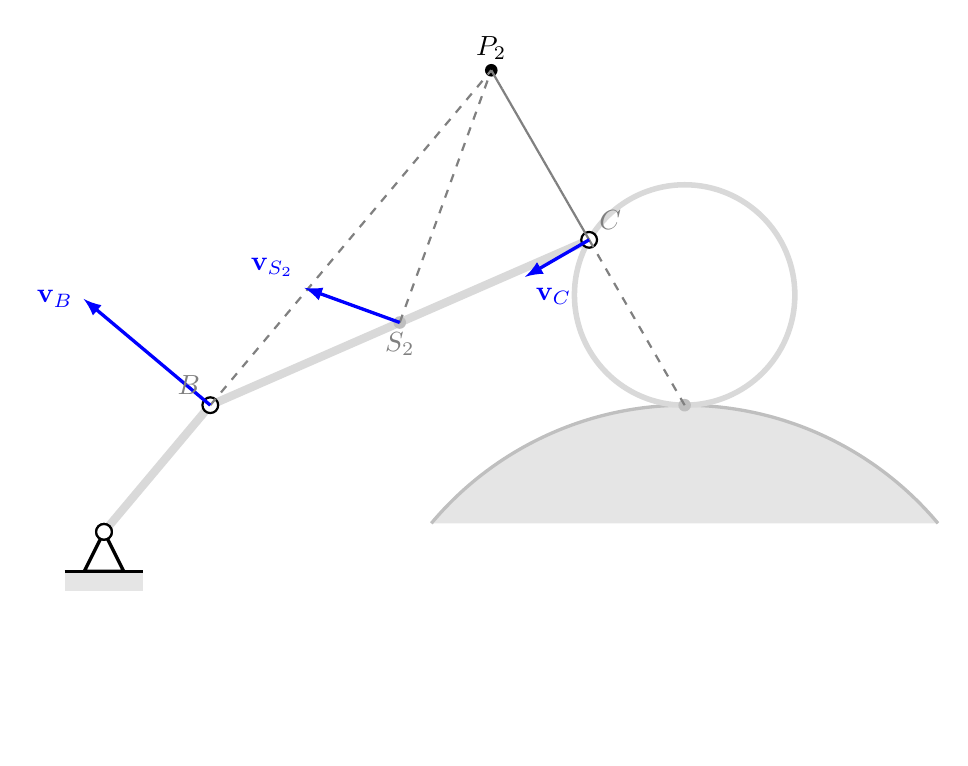
\begin{tikzpicture}[>=Stealth, thick]
    \def\sc{35}
    \def\vsc{7} % Sebesség vektor skálázása
    
    \coordinate (A) at (0*\sc, 0*\sc);
    \coordinate (B) at (0.03857*\sc, 0.04596*\sc);
    \coordinate (C) at (0.17604*\sc, 0.10596*\sc);
    \coordinate (S3) at (0.21069*\sc, 0.08596*\sc);
    \coordinate (K) at (0.21069*\sc, 0.04596*\sc);
    \coordinate (S2) at (0.10731*\sc, 0.07596*\sc);
    \coordinate (Ocyl) at (0.21069*\sc, -0.07404*\sc);
    \coordinate (P2) at (0.14053*\sc, 0.16748*\sc);
    
    % Vektorok
    \coordinate (vB) at (-0.22981*\vsc, 0.19284*\vsc);
    \coordinate (vC) at (-0.11634*\vsc, -0.06717*\vsc);
    \coordinate (vS2) at (-0.17308*\vsc, 0.06283*\vsc);
    
    % Henger
    \draw[very thick, fill=gray!20, draw=gray!50] (Ocyl) ++(140:0.12*\sc) arc[start angle=140, end angle=40, radius=0.12*\sc];

    % Szerkezet halványan
    \draw[line width=3pt, gray!30] (A) -- (B) -- (C);
    \draw[line width=2pt, gray!30, fill=white] (S3) circle (0.04*\sc);
    
    \supporthinge[draw=gray!50]{A}{0}
    \hinge[draw=gray!50]{A}
    \hinge[draw=gray!50]{B}
    \hinge[draw=gray!50]{C}
    \fill[gray!50] (S2) circle (0.08);
    \fill[gray!50] (K) circle (0.08);
    
    % P2 és vonalak
    \fill[black] (P2) circle (0.08) node[above] {$P_2$};
    \draw[dashed, gray] (B) -- (P2);
    \draw[dashed, gray] (C) -- (P2);
    \draw[dashed, gray] (K) -- (P2);
    \draw[dashed, gray] (S2) -- (P2);
    
    % Sebességvektorok
    \draw[vec=blue] (B) -- ($(B) + (vB)$) node[left] {$\vec{v}_B$};
    \draw[vec=blue] (C) -- ($(C) + (vC)$) node[below right] {$\vec{v}_C$};
    \draw[vec=blue] (S2) -- ($(S2) + (vS2)$) node[above left] {$\vec{v}_{S_2}$};
    
    % Pontok jelölése
    \node[above left, gray] at (B) {$B$};
    \node[above right, gray] at (C) {$C$};
    \node[below, gray] at (S2) {$S_2$};
\end{tikzpicture}

    \caption{Sebességvektorok és a sebességpólus ($P_2$) helyzete}
\end{figure}

\section{Gyorsulásállapot vizsgálata (4., 5., 6. feladat)}
\subsection{A (2) test szöggyorsulása és az $S_2$ pont gyorsulása (4. feladat)}
Az 1-es rúd B pontjának gyorsulása (mivel $\vec{\omega}_1 = \text{állandó}$, így $\vec{v}_B = \vec{v}_{Bn}$):
\begin{equation}
    \vec{a}_B = -\omega_1^2 \vec{r}_{AB} = \begin{bmatrix} -0,9642 \\ -1,1491 \\ 0 \end{bmatrix} \text{ m/s}^2
\end{equation}

A (2) rúdon a C pont gyorsulása kifejezhető a B pontból relatív gyorsulással:
\begin{equation}
    \vec{a}_C = \vec{a}_B + \vec{\varepsilon}_2 \times \vec{r}_{BC} - \omega_2^2 \vec{r}_{BC} \label{eq:ac_from_b}
\end{equation}

A (3) kerék tiszta gördülést végez egy $R=3r_3$ sugarú hengerfelületen. A kerék $S_3$ súlypontja így $R+r_3$ sugarú körpályán mozog, ezért normális gyorsulása (mely a görbületi középpont felé mutat):
\begin{equation}
    a_{S_3, n} = \frac{v_{S_3}^2}{R+r_3}
\end{equation}
A C pont gyorsulása kifejezhető a 3-as kerék $S_3$ pontjából is:
\begin{equation}
    \vec{a}_C = \vec{a}_{S_3} + \vec{\varepsilon}_3 \times \vec{r}_{S_3 C} - \omega_3^2 \vec{r}_{S_3 C} \label{eq:ac_from_s3}
\end{equation}
A \eqref{eq:ac_from_b} és \eqref{eq:ac_from_s3} egyenletek egyenlővé tételével egy 2 ismeretlenes ($\varepsilon_{2z}$, $\varepsilon_{3z}$) lineáris egyenletrendszert kapunk az $x$ és $y$ komponensekre. Ennek megoldása adja a keresett szöggyorsulásokat: $\varepsilon_{2z} = 1,9471 \text{ rad/s}^2$ és $\varepsilon_{3z} = 28,3829 \text{ rad/s}^2$.

Az $S_2$ pont gyorsulása az aszimmetrikus (2) test B pontjából:
\begin{equation}
    \vec{a}_{S_2} = \vec{a}_B + \vec{\varepsilon}_2 \times \vec{r}_{BS_2} - \omega_2^2 \vec{r}_{BS_2} = \begin{bmatrix} -1,2685 \\ -1,1225 \\ 0 \end{bmatrix} \text{ m/s}^2, \quad |\vec{a}_{S_2}| = 1,6938 \text{ m/s}^2
\end{equation}

\subsection{Gyorsulásvektorok (5. feladat)}
\begin{figure}[H]
    \centering
    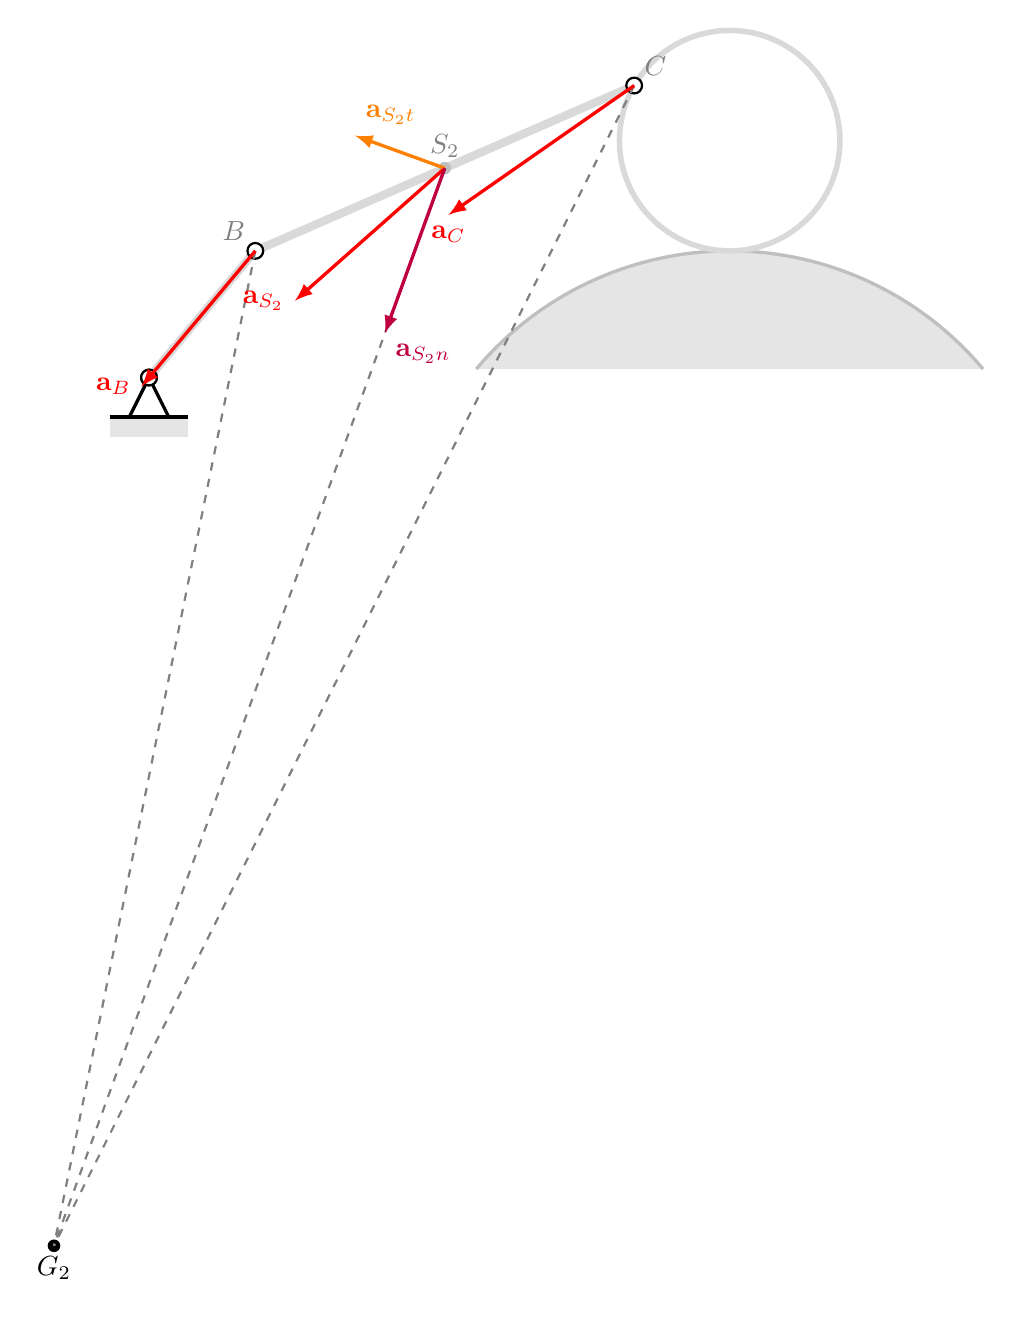
\begin{tikzpicture}[>=Stealth, thick]
    \def\sc{35}
    \def\asc{1.5} % Gyorsulás vektor skálázása
    
    \coordinate (A) at (0*\sc, 0*\sc);
    \coordinate (B) at (0.03857*\sc, 0.04596*\sc);
    \coordinate (C) at (0.17604*\sc, 0.10596*\sc);
    \coordinate (S3) at (0.21069*\sc, 0.08596*\sc);
    \coordinate (K) at (0.21069*\sc, 0.04596*\sc);
    \coordinate (S2) at (0.10731*\sc, 0.07596*\sc);
    \coordinate (Ocyl) at (0.21069*\sc, -0.07404*\sc);
    
    \coordinate (G2) at (-0.03448*\sc, -0.31505*\sc);
    
    % Vektorok
    \coordinate (aB) at (-0.96418*\asc, -1.14907*\asc);
    \coordinate (aC) at (-1.57274*\asc, -1.09600*\asc);
    \coordinate (aS2) at (-1.26846*\asc, -1.12253*\asc);
    \coordinate (aS2t) at (-0.76067*\asc, 0.27616*\asc);
    \coordinate (aS2n) at (-0.50779*\asc, -1.39869*\asc);
    
    % Henger
    \draw[very thick, fill=gray!20, draw=gray!50] (Ocyl) ++(140:0.12*\sc) arc[start angle=140, end angle=40, radius=0.12*\sc];

    % Szerkezet halványan
    \draw[line width=3pt, gray!30] (A) -- (B) -- (C);
    \draw[line width=2pt, gray!30, fill=white] (S3) circle (0.04*\sc);
    
    \supporthinge[draw=gray!50]{A}{0}
    \hinge[draw=gray!50]{A}
    \hinge[draw=gray!50]{B}
    \hinge[draw=gray!50]{C}
    \fill[gray!50] (S2) circle (0.08);
    
    % Gyorsuláspólus
    \fill[black] (G2) circle (0.08) node[below] {$G_2$};
    \draw[dashed, gray] (B) -- (G2);
    \draw[dashed, gray] (C) -- (G2);
    \draw[dashed, gray] (S2) -- (G2);
    
    % Gyorsulásvektorok
    \draw[vec=red] (B) -- ($(B) + (aB)$) node[left] {$\vec{a}_B$};
    \draw[vec=red] (C) -- ($(C) + (aC)$) node[below] {$\vec{a}_C$};
    \draw[vec=red] (S2) -- ($(S2) + (aS2)$) node[left] {$\vec{a}_{S_2}$};
    
    % Komponensek
    \draw[vec=orange] (S2) -- ($(S2) + (aS2t)$) node[above right] {$\vec{a}_{S_2t}$};
    \draw[vec=purple] (S2) -- ($(S2) + (aS2n)$) node[below right] {$\vec{a}_{S_2n}$};

    % Pontok jelölése
    \node[above left, gray] at (B) {$B$};
    \node[above right, gray] at (C) {$C$};
    \node[above, gray] at (S2) {$S_2$};
\end{tikzpicture}

    \caption{Gyorsulásvektorok}
\end{figure}

\subsection{Gyorsulásszög és gyorsuláspólus (6. feladat)}
A (2) test gyorsulásszöge az iránytangens alapján:
\begin{equation}
    \alpha_2 = \arctan \left( \frac{|\varepsilon_2|}{\omega_2^2} \right) = 28,56^\circ
\end{equation}
A gyorsuláspólus ($G_2$) helyvektora a B pontból számítva, a képlet alapján:
\begin{equation}
    \vec{r}_{BG_2} = \frac{\omega_2^2 \vec{a}_B + \vec{\varepsilon}_2 \times \vec{a}_B}{\omega_2^4 + \varepsilon_2^2} \implies G_2(-0,0345; -0,3151) \text{ m}
\end{equation}

\section{Pálya jellemzői (7., 8. feladat)}
\subsection{Érintő és normális gyorsulás komponensek (7. feladat)}
Az $S_2$ pont pályamenti érintő (tangenciális) egységvektora a sebesség iránya:
\begin{equation}
    \vec{e}_t = \frac{\vec{v}_{S_2}}{|\vec{v}_{S_2}|}
\end{equation}
Ezzel a tangenciális gyorsuláskomponens nagysága és vektora skaláris szorzatként:
\begin{equation}
    a_{S_2, t} = \vec{a}_{S_2} \cdot \vec{e}_t = 0,8093 \text{ m/s}^2, \quad \vec{a}_{S_2, t} = \begin{bmatrix} -0,7607 \\ 0,2762 \\ 0 \end{bmatrix} \text{ m/s}^2
\end{equation}
A normális gyorsuláskomponens vektorkivonással adódik:
\begin{equation}
    \vec{a}_{S_2, n} = \vec{a}_{S_2} - \vec{a}_{S_2, t} = \begin{bmatrix} -0,5078 \\ -1,3987 \\ 0 \end{bmatrix} \text{ m/s}^2, \quad |\vec{a}_{S_2, n}| = 1,4880 \text{ m/s}^2
\end{equation}

\subsection{Görbületi sugár (8. feladat)}
Az $S_2$ pont pályájának görbületi sugara a normális gyorsulás és a sebesség összefüggéséből számítható:
\begin{equation}
    \rho_{S_2} = \frac{|\vec{v}_{S_2}|^2}{|\vec{a}_{S_2, n}|} = 0,0228 \text{ m}
\end{equation}

\end{document}
